\ChapterImageStar[cap:pmv]{Producto Mínimo Viable}{./images/fondo.png}\label{cap:pmv}
\mbox{}\\
En este capítulo se implementará el sistema propuesto en la infraestructura HTCondor del Grupo \GRID. Además, se enunciarán las características de cada componente del sistema, su contenido, requisitos y guía de instalación, para hacer un entorno repetible y escalable.

Cabe destacar que para este proyecto se usó Git para el control de versiones, GitHub para gestión de repositorios y se usó un enfoque hacia versionamiento semántico o \textit{SemVer}. Por lo que se mostrarán las aplicaciones y se mencionará la última versión funcional de la aplicación con un \textit{tag}.

\section{\textit{Grid App}}
\noindent
Como se mencionó en el capítulo de diseño de la solución, la aplicación \textit{Grid App} constituye la piedra angular del sistema, funcionando como la interfaz central que permite a los usuarios interactuar con la infraestructura HTCondor distribuida. Esta aplicación web desarrollada en Flask permite cargar trabajos computacionales, configurar parámetros de ejecución específicos para diferentes tipos de universos HTCondor, y visualizar los resultados de manera organizada y accesible.

\subsection{Estructura del proyecto}
\noindent
La aplicación \textit{Grid App} está organizada siguiendo las mejores prácticas de desarrollo web con Flask:

\begin{itemize}
	\item \textbf{app.py}: Archivo principal que contiene la lógica del servidor Flask, incluyendo todos los \textit{endpoints}, manejo de archivos, generación de \textit{submit files} y lógica de interacción con HTCondor.

	\item \textbf{templates/}: Directorio que contiene las plantillas \HTML para la interfaz de usuario:
	      \begin{itemize}
		      \item \texttt{upload.html}: Interfaz principal para la carga y configuración de trabajos.
		      \item \texttt{results.html}: Interfaz para visualización de resultados con sistema de pestañas dinámicas.
	      \end{itemize}

	\item \textbf{static/}: Directorio para archivos estáticos (CSS, JavaScript, imágenes) que proporcionan estilo e interactividad a la aplicación web.

	\item \textbf{submits/}: Directorio de trabajo donde se almacenan todos los archivos relacionados con cada trabajo:
	      \begin{itemize}
		      \item Archivos ejecutables subidos por el usuario.
		      \item Archivos de entrada (para trabajos paralelos).
		      \item \textit{Submit files} generados automáticamente.
		      \item Archivos de salida y \textit{logs} de HTCondor.
		      \item Metadatos del trabajo en formato \JSON.
	      \end{itemize}

	\item \textbf{scripts/}: Directorio que contiene scripts auxiliares de Bash para operaciones específicas:
	      \begin{itemize}
		      \item \texttt{send-submit.sh}: Envío de trabajos a clústeres remotos vía SSH.
		      \item \texttt{fetch-outputs.sh}: Sincronización de archivos de salida desde clústeres remotos.
	      \end{itemize}
\end{itemize}

\begin{figure}[H]
	\centering
	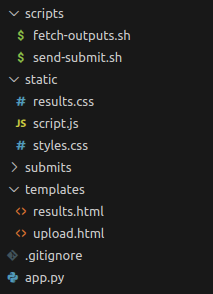
\includegraphics[scale=0.7]{tablas-images/pmv/estructura-proyecto-grid-app.png}
	\caption{Estructura del proyecto \textit{Grid App}}
	\label{fig:estructura-proyecto-grid-app}
\end{figure}

\subsection{Código fuente}
\noindent

% TODO: Actualizar información del repositorio, rama y versión
El código fuente de la aplicación \textit{Grid App} está disponible en el repositorio correspondiente y su implementación se presenta en los apéndices de este documento. La aplicación está desarrollada completamente en Python utilizando el \textit{framework} Flask para el \textit{backend} y HTML/CSS/JavaScript para la interfaz de usuario.

\subsection{Características técnicas y configuración}
\noindent

\subsubsection{Configuración de la aplicación}
\noindent

La aplicación \textit{Grid App} utiliza las siguientes configuraciones globales definidas en \texttt{app.py}:

\begin{itemize}
	\item \textbf{DEFAULT\_PROJECT\_FOLDER}: Directorio base de la aplicación, configurable entre desarrollo y producción.
	\item \textbf{SUBMIT\_FOLDER}: Directorio para almacenamiento de trabajos (\texttt{/submits/}).
	\item \textbf{SCRIPTS\_FOLDER}: Directorio de scripts auxiliares (\texttt{/scripts/}).
	\item \textbf{JOB\_STATUS}: Diccionario global para traducción de códigos de estado HTCondor.
\end{itemize}

\subsubsection{Manejo de archivos y permisos}
\noindent

El sistema implementa un manejo robusto de archivos:

\begin{itemize}
	\item \textbf{Permisos ejecutables}: Los archivos binarios reciben permisos \texttt{0o755} automáticamente.
	\item \textbf{Codificación de archivos}: Lectura de salidas con \texttt{encoding='utf-8', errors='ignore'}.
	\item \textbf{Gestión de directorios}: Creación automática con \texttt{os.makedirs(job\_dir, exist\_ok=True)}.
\end{itemize}

\subsubsection{Concurrencia y \textit{multithreading}}
\noindent

Para trabajos paralelos, la aplicación utiliza \textit{threading} para operaciones no bloqueantes:

\begin{verbatim}
def traer_salidas():
    subprocess.run(['./fetch-outputs.sh', job_dir, submit_ip, job_id], ...)

thread = threading.Thread(target=traer_salidas)
thread.start()
\end{verbatim}

\subsection{Componentes de la interfaz web}
\noindent

\subsubsection{\textit{Upload Interface}}
\noindent
Interfaz principal implementada en \texttt{upload.html}, servida por el \textit{endpoint} raíz. Proporciona un formulario \textit{multipart} para carga de archivos y configuración de parámetros de ejecución específicos por tipo de universo HTCondor.

\begin{figure}[H]
	\centering
	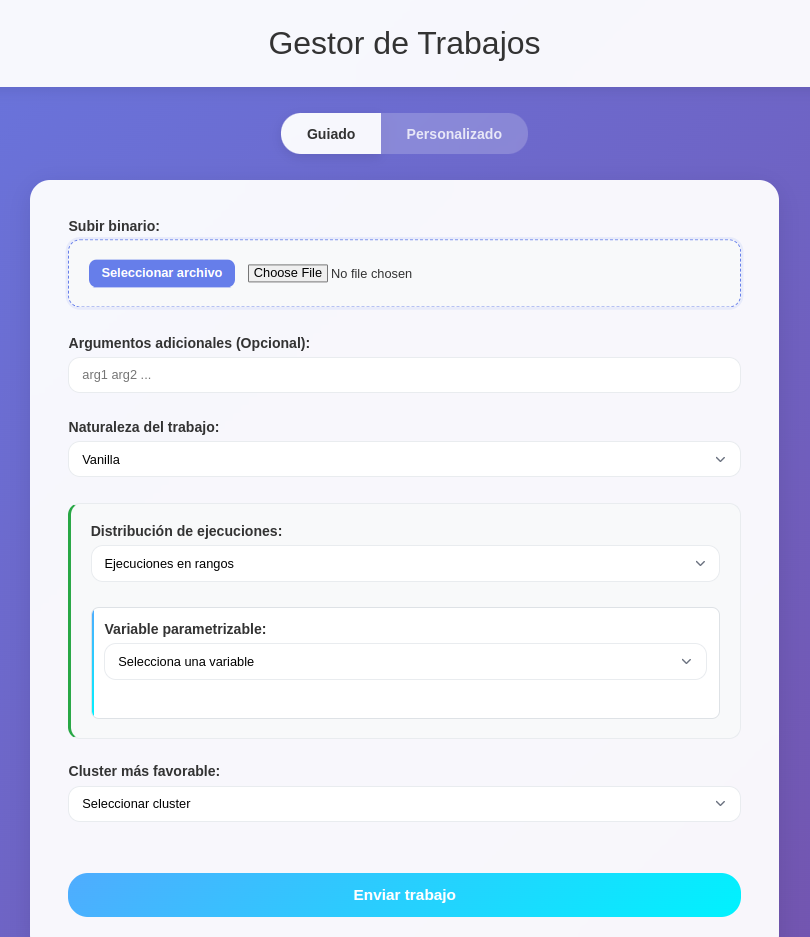
\includegraphics[scale=0.5]{tablas-images/pmv/upload-ui-screenshot.png}
	\caption{Interfaz de carga de trabajos}
	\label{fig:uiCargasTrabajos}
\end{figure}

\subsubsection{\textit{Results Interface}}
\noindent
Interfaz dinámica implementada en \texttt{results.html} que utiliza JavaScript para carga asíncrona de archivos de salida mediante peticiones AJAX al \textit{endpoint} \texttt{/output/<job\_id>/<filename>}. Presenta información completa del trabajo y sistema de pestañas para navegación entre múltiples archivos de salida.

\begin{figure}[H]
	\centering
	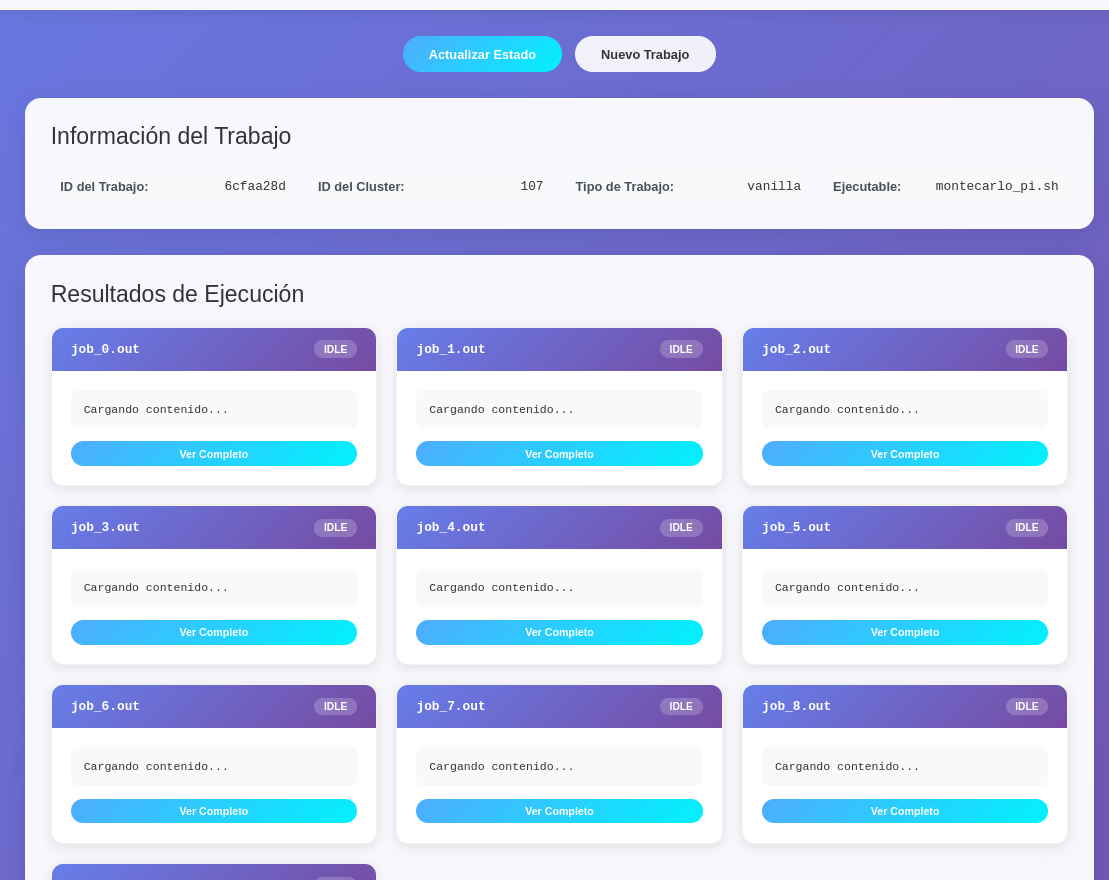
\includegraphics[scale=0.35]{tablas-images/pmv/results-ui-screenshot.png}
	\caption{Interfaz de resultados de trabajos}
	\label{fig:uiResultadosTrabajos}
\end{figure}

\subsection{Componentes \textit{backend} (\textit{endpoints})}
\noindent

La aplicación \textit{Grid App} está implementada como una aplicación Flask que expone múltiples \textit{endpoints} para gestionar el ciclo de vida completo de los trabajos computacionales en HTCondor. El servidor Flask se ejecuta por defecto en el puerto \texttt{5000} y está configurado para aceptar conexiones desde cualquier interfaz de red (\texttt{host='0.0.0.0'}). Los \textit{endpoints} principales del sistema se describen a continuación.

\subsubsection{Root Endpoint (/)}
\noindent

El \textit{Root Endpoint} sirve la página principal de la aplicación. Este \textit{endpoint} está expuesto en la ruta raíz (\texttt{/}) y acepta peticiones de tipo GET.

\textbf{Funcionamiento:}

Renderiza la plantilla HTML \texttt{upload.html} que contiene la interfaz principal para la carga y configuración de trabajos computacionales.

\subsubsection{Submit Endpoint (/submit)}
\noindent

El \textit{Submit Endpoint} es el componente más complejo del sistema, responsable de procesar la información del trabajo computacional y coordinarlo con los diferentes tipos de universos HTCondor. Este \textit{endpoint} está expuesto en la ruta \texttt{/submit} y acepta peticiones de tipo \texttt{POST}.

\textbf{Funcionamiento:}

\begin{enumerate}
	\item \textbf{Generación del identificador único}: Genera un UUID de 8 caracteres utilizando \texttt{str(uuid.uuid4())[:8]} para identificar únicamente cada trabajo.

	\item \textbf{Procesamiento de archivos}: Recibe y procesa hasta tres archivos opcionales del formulario multipart:
	      \begin{itemize}
		      \item \texttt{binary-file}: Ejecutable principal del trabajo.
		      \item \texttt{input-file}: Archivo de entrada (requerido para trabajos parallel).
		      \item \texttt{submit-file}: Submit file personalizado de HTCondor.
	      \end{itemize}

	\item \textbf{Configuración del trabajo}: Parsea la configuración JSON que incluye:
	      \begin{itemize}
		      \item \texttt{jobType}: Especifica el universo (\texttt{'vanilla'} o \texttt{'parallel'}).
		      \item \texttt{cluster}: Dirección del clúster de destino.
		      \item \texttt{additionalArgs}: Argumentos para el ejecutable.
		      \item \texttt{vanillaMode}: Modo de distribución para trabajos vanilla ('range' o 'equal').
		      \item \texttt{rangeOptions}: Configuración de variables y rangos.
		      \item \texttt{parallelOptions}: Configuración de máquinas y núcleos.
	      \end{itemize}

	\item \textbf{Generación automática de submit files}: La función \texttt{create\_submit\_file()} genera diferentes tipos de submit files:

	      \textbf{Para universo Grid (Vanilla):}
	      \begin{itemize}
		      \item Configura \texttt{universe = grid} y \texttt{grid\_resource = condor}.
		      \item Establece requisitos de arquitectura: \texttt{requirements = (Arch == ``armv7l'')}.
		      \item Maneja distribución de trabajos:
		            \begin{itemize}
			            \item \textit{Modo range}: Genera trabajos explícitos con variables iterativas.
			            \item \textit{Modo equal}: Crea trabajos idénticos con \texttt{queue N}.
		            \end{itemize}
	      \end{itemize}

	      \textbf{Para universo Parallel:}
	      \begin{itemize}
		      \item Configura \texttt{universe = parallel}.
		      \item Utiliza \texttt{executable = /usr/share/doc/condor/examples/openmpiscript}.
		      \item Establece \texttt{machine\_count} y \texttt{request\_cpus}.
		      \item Configura variables de entorno OpenMPI.
		      \item Establece política de apagado: \texttt{+ParallelShutdownPolicy = ``WAIT\_FOR\_NODE0''}.
	      \end{itemize}

	\item \textbf{Ejecución de trabajos}:

	      \textbf{Trabajos Vanilla:} Ejecuta \texttt{condor\_submit} directamente en el directorio local del trabajo.

	      \textbf{Trabajos Parallel:}
	      \begin{itemize}
		      \item Ejecuta el script \texttt{send-submit.sh} para transferir archivos al clúster remoto.
		      \item Inicia un hilo separado con \texttt{threading.Thread} que ejecuta \texttt{fetch-outputs.sh}.
	      \end{itemize}

	\item \textbf{Extracción del cluster ID}: Utiliza la expresión regular \texttt{r``(\\textbackslash{}d+)\\textbackslash{}s+job\\textbackslash{}(s\\textbackslash{})\\textbackslash{}s+submitted to cluster\\textbackslash{}s+(\\textbackslash{}d+)''} para extraer el ID del clúster de la salida de \texttt{condor\_submit}.

	\item \textbf{Persistencia de metadatos}: Guarda \texttt{job\_info.json} con información completa del trabajo, incluyendo configuración, timestamps y salida de HTCondor.
\end{enumerate}

\textbf{Respuesta:}

Retorna un JSON con la estructura:

\begin{verbatim}
{
  "success": true,
  "job_id": "a1b2c3d4", 
  "cluster_id": "123",
  "message": "Trabajo enviado exitosamente"
}
\end{verbatim}

\subsubsection{Job Status Endpoint (/job\_status/<job\_id>)}
\noindent

Este endpoint consulta el estado actual de un trabajo en los sistemas HTCondor correspondientes, manejando tanto trabajos locales (vanilla) como remotos (parallel).

\textbf{Funcionamiento:}

\begin{enumerate}
	\item \textbf{Validación}: Verifica la existencia de \texttt{job\_info.json} y extrae el \texttt{cluster\_id}.

	\item \textbf{Consulta de estado}: Ejecuta comandos específicos según el tipo de trabajo:

	      \textbf{Trabajos Vanilla:}
	      \begin{verbatim}
condor_q {cluster_id} -long | grep -E '^JobStatus'
	      \end{verbatim}

	      \textbf{Trabajos Parallel:}
	      \begin{verbatim}
ssh -i ~/.ssh/parallel alma@{submit_ip} 
  "condor_q {cluster_id} -long | grep -E '^JobStatus'"
	      \end{verbatim}

	\item \textbf{Consulta en historial}: Si no se encuentra en \texttt{condor\_q}, consulta \texttt{condor\_history} con \texttt{-limit 1}.

	\item \textbf{Procesamiento de estados}: Utiliza el diccionario global \texttt{JOB\_STATUS} para traducir códigos numéricos:

	      \begin{table}[H]
		      \centering
		      \begin{tabular}{|c|l|}
			      \hline
			      \textbf{Código} & \textbf{Estado} \\
			      \hline
			      1               & Idle            \\
			      2               & Running         \\
			      3               & Removed         \\
			      4               & Completed       \\
			      5               & Held            \\
			      \hline
		      \end{tabular}
		      \caption{Códigos de estado de HTCondor}
		      \label{tab:job-status-codes}
	      \end{table}

	\item \textbf{Determinación del estado general}:
	      \begin{itemize}
		      \item \texttt{all(s == ``Completed'' for s in statuses)}: Estado ``Completed''.
		      \item \texttt{``Running'' in statuses}: Estado ``Running''.
		      \item \texttt{len(set(statuses)) > 1}: Estado ``Mixed''.
		      \item Caso contrario: Primer estado de la lista.
	      \end{itemize}
\end{enumerate}

\textbf{Respuesta:}

\begin{verbatim}
{
  "job_id": "a1b2c3d4",
  "cluster_id": "123", 
  "statuses": ["Running", "Completed"],
  "overall_status": "Running"
}
\end{verbatim}

\subsubsection{Results Endpoint (/results/<job\_id>)}
\noindent

Este endpoint renderiza la página de visualización de resultados con un sistema dinámico de pestañas para múltiples archivos de salida.

\textbf{Funcionamiento:}

\begin{enumerate}
	\item \textbf{Validación}: Verifica la existencia del directorio del trabajo.

	\item \textbf{Carga de metadatos}: Lee \texttt{job\_info.json} para obtener la configuración del trabajo.

	\item \textbf{Identificación de archivos de salida}:

	      \textbf{Trabajos Vanilla:}
	      \begin{verbatim}
for filename in os.listdir(job_dir):
    if filename.startswith('job_') and filename.endswith('.out'):
        output_files.append(filename)
output_files.sort()
	      \end{verbatim}

	      \textbf{Trabajos Parallel:}
	      \begin{verbatim}
output_files = ['job_0.out']
	      \end{verbatim}

	\item \textbf{Renderizado}: Utiliza \texttt{render\_template('results.html')} con contexto que incluye \texttt{job\_info}, \texttt{output\_files} y \texttt{job\_id}.
\end{enumerate}

\subsubsection{Output Endpoint (/output/<job\_id>/<filename>)}
\noindent

Endpoint auxiliar que sirve el contenido específico de archivos de salida individuales para carga dinámica mediante AJAX.

\textbf{Funcionamiento:}

\begin{enumerate}
	\item \textbf{Construcción de ruta}: \texttt{os.path.join(job\_dir, filename)}

	\item \textbf{Validación}: \texttt{os.path.exists(output\_path)}

	\item \textbf{Lectura robusta}:
	      \begin{verbatim}
with open(output_path, 'r') as file:
    content = file.read()
	      \end{verbatim}

	\item \textbf{Respuesta}: \texttt{Response(content, mimetype='text/plain')}
\end{enumerate}

\subsubsection{State Endpoint (/state/<id>)}
\noindent

Endpoint simplificado para consulta rápida de estado por clúster ID (funcionalidad adicional).

\textbf{Funcionamiento:}

Ejecuta \texttt{condor\_q \{id\} -long | grep -E '\^{}JobStatus'} y retorna directamente el estado traducido usando el diccionario \texttt{JOB\_STATUS}.

\subsection{Proceso de instalación}
\noindent

\subsubsection{Descripción general del entorno}
\noindent
Requisitos del sistema para el despliegue de \textit{Grid App}:

\begin{itemize}
	\item Sistema operativo: Raspbian GNU/Linux 9 (stretch) o superior.
	\item Python: Versión 3.6 o superior con pip.
	\item Dependencias Python: Flask y módulos estándar (uuid, threading, subprocess).
	\item HTCondor: Instalación completa con universo Grid configurado.
	\item SSH: Configuración de claves para acceso a clústeres remotos (parallel jobs).
	\item Usuario: Permisos para ejecutar comandos HTCondor y escritura en directorios de trabajo.
\end{itemize}

\subsubsection{Pasos de instalación}
\noindent

% TODO: Actualizar URL del repositorio, rama y comandos de instalación específicos
Instalación de la aplicación:

\begin{enumerate}
	\item Clonar el repositorio:
	      \begin{verbatim}
			git clone [URL_REPOSITORIO] /opt/grid-app
		\end{verbatim}

	\item Instalar dependencias Python:
	      \begin{verbatim}
			cd /opt/grid-app
			pip3 install flask
		\end{verbatim}

	\item Configurar directorios de trabajo:
	      \begin{verbatim}
			mkdir -p /opt/grid-app/submits
			mkdir -p /opt/grid-app/scripts
			chmod 755 /opt/grid-app/scripts/*.sh
		\end{verbatim}

	\item Configurar acceso SSH para trabajos parallel:
	      \begin{verbatim}
			ssh-keygen -t rsa -f ~/.ssh/parallel
			# Copiar clave pública a clústeres remotos
		\end{verbatim}
\end{enumerate}

\subsubsection{Configuración del servicio}
\noindent

Para ejecutar la aplicación como servicio del sistema:

% !TODO: Crear script de instalación automatizado similar al de Cluster Info App
\begin{enumerate}
	\item Crear archivo de unidad systemd en \texttt{/etc/systemd/system/grid-app.service}.
	\item Configurar el servicio para ejecutarse en el puerto 5000.
	\item Habilitar y iniciar el servicio con systemctl.
\end{enumerate}

\subsubsection{Mantenimiento automático}
\noindent

Configuración de limpieza periódica del directorio de trabajos:

\begin{enumerate}
	\item Agregar al crontab:
	      \begin{verbatim}
			crontab -e
		\end{verbatim}

	\item Agregar tarea de limpieza diaria:
	      \begin{verbatim}
			0 2 * * * find /opt/grid-app/submits \
				-type d -mtime +7 -exec rm -rf {} +
		\end{verbatim}
\end{enumerate}

La configuración presentada representa el entorno específico utilizado durante el desarrollo y puede requerir adaptaciones según las características particulares del sistema de destino y los requisitos de la infraestructura HTCondor existente.

\section{\textit{Cluster Info App}}
\noindent

Como se mencionó en el capítulo de diseño de la solución, la aplicación \textit{Cluster Info App} es la encargada de recopilar métricas del clúster y exponerlas a través de una \API. Es importante añadir que esta aplicación debe correr en la máquina \textit{submit} de cada clúster al que se quieran enviar trabajos, pues es a través de esta que el \textit{grid manager} y la aplicación \textit{Grid App} obtienen la información para redirigir los trabajos y ejecutarlos en los recursos remotos.

\subsection{Estructura del proyecto}
\noindent
La aplicación \textit{Cluster Info App} está compuesta por tres archivos principales que trabajan en conjunto para proporcionar métricas del clúster HTCondor:

\begin{itemize}
	\item \textbf{update\_condor\_metrics.sh}: \textit{Script} de \textit{Bash} que recopila métricas del clúster HTCondor ejecutando comandos específicos de HTCondor y generando un archivo JSON con la información.
	\item \textbf{cluster-info.py}: Servidor HTTP ligero implementado en Python que lee las métricas del archivo JSON y las expone a través de una API REST.
	\item \textbf{install.sh}: \textit{Script} de instalación que configura el servicio como un daemon del sistema usando systemd.
\end{itemize}

\begin{figure}[H]
	\centering
	
\includegraphics[scale=0.7]{tablas-images/pmv/estructura-proyecto-cluster-info-app.png}
	\caption{Estructura del proyecto \textit{Cluster Info App}}
	\label{fig:estructura-proyecto-cluster-info-app}
\end{figure}

\subsection{Componentes de la aplicación}
\noindent

\subsubsection{Script de recopilación de métricas (update\_condor\_metrics.sh)}
\noindent

Este componente es responsable de ejecutar comandos específicos de HTCondor para recopilar información del estado del clúster y generar un archivo JSON con las métricas. El \textit{script} recopila las siguientes métricas:

\begin{itemize}
	\item \textbf{Slots disponibles}: Utiliza el comando \texttt{condor\_status -avail -total} para obtener el número total de \textit{slots} de CPU disponibles en el clúster.

	\item \textbf{Porcentaje de trabajos exitosos}: Calcula el porcentaje de trabajos completados exitosamente mediante el análisis del historial de trabajos con \texttt{condor\_history}.

	\item \textbf{Trabajos en cola}: Extrae el número de trabajos inactivos (\textit{idle}) usando \texttt{condor\_q}.

	\item \textbf{Direcciones del sistema}: Obtiene las direcciones IP del \textit{collector} y \textit{schedd} mediante consultas a los \textit{daemons} correspondientes.

	\item \textbf{Tipo de clúster}: Identifica el tipo de universo soportado por el clúster (en este caso, Vanilla).
\end{itemize}

El resultado se almacena en el archivo \texttt{/tmp/condor\_metrics.json} con el siguiente formato:

\begin{verbatim}
{
  "slots": "8",
  "success_jobs": "95%",
  "idle_jobs": "3",
  "collector_address": "192.168.1.100:9618",
  "schedd_address": "192.168.1.100:9615",
  "cluster_type": "vanilla"
}
\end{verbatim}

\subsubsection{Servidor HTTP (cluster-info.py)}
\noindent

Este componente implementa un servidor HTTP ligero utilizando la librería estándar de Python \texttt{http.server}. El servidor expone las métricas del clúster a través de una API REST simple.

\textbf{Características principales:}

\begin{itemize}
	\item \textbf{Puerto de servicio}: El servidor se ejecuta en el puerto 44444 por defecto.

	\item \textbf{Endpoint principal}: Responde a peticiones GET en la ruta raíz (\texttt{/}) devolviendo las métricas en formato JSON.

	\item \textbf{Soporte CORS}: Incluye cabeceras CORS para permitir peticiones desde diferentes dominios, facilitando la integración con aplicaciones web.

	\item \textbf{Manejo de errores}: Implementa manejo de excepciones devolviendo respuestas HTTP 500 con información del error en formato JSON.

	\item \textbf{Soporte para preflight requests}: Maneja peticiones OPTIONS para cumplir con los requisitos de CORS.
\end{itemize}

\textbf{Funcionamiento:}

\begin{enumerate}
	\item El servidor lee el archivo \texttt{/tmp/condor\_metrics.json} generado por el \textit{script} de métricas.
	\item Procesa la información y la devuelve como respuesta JSON.
	\item En caso de error (archivo no encontrado, formato incorrecto, etc.), devuelve un mensaje de error estructurado.
\end{enumerate}

\subsubsection{Script de instalación (install.sh)}
\noindent

Este componente automatiza el proceso de instalación y configuración de la aplicación como un servicio del sistema. El \textit{script} realiza las siguientes operaciones:

\begin{itemize}
	\item \textbf{Verificación de privilegios}: Valida que se ejecute con permisos de superusuario.

	\item \textbf{Instalación de dependencias}: Actualiza el sistema e instala Python 3 y pip usando el gestor de paquetes APT.

	\item \textbf{Configuración de systemd}: Crea un archivo (\texttt{cluster-info.service}) que define el servicio con las siguientes características:
	      \begin{itemize}
		      \item Ejecuta bajo el usuario \texttt{pi}.
		      \item Configura reinicio automático en caso de falla.
		      \item Redirige la salida al journal del sistema.
		      \item Se ejecuta después de que la red esté disponible.
	      \end{itemize}

	\item \textbf{Habilitación del servicio}: Recarga el daemon de systemd, habilita el servicio para inicio automático y lo pone en marcha.

	\item \textbf{Verificación}: Muestra el estado del servicio para confirmar que la instalación fue exitosa.
\end{itemize}

\subsection{Código fuente}
\noindent

El código fuente de la aplicación \textit{Cluster Info App} está disponible en el repositorio correspondiente y su implementación se presenta en los apéndices de este documento. La aplicación está diseñada para ser ligera, confiable y fácil de desplegar en diferentes entornos de HTCondor.

\subsection{Proceso de instalación}
\noindent

Con el fin de hacer el proceso repetible se preparó una descripción general del entorno y una serie de pasos para la instalación de la aplicación

\subsubsection{Descripción general del entorno}
\noindent
A continuación se muestran algunas de las condiciones que cumple el entorno en el que se instaló la aplicación para que esta pudiera funcionar

\begin{itemize}
	\item Sistema operativo: Raspbian GNU/Linux 9 (stretch).
	\item Gestor de paquetes: APT.
	\item Usuario: pi.
	\item Grupos: pi, sudo.
	\item Herramientas adicionales: Git, Condor, Python3 y Grid Universe instalado.
\end{itemize}

\subsubsection{Pasos}
\noindent

Instalación de la aplicación:

\begin{enumerate}
	\item Clonar el repositorio:
	      \begin{verbatim}
			git clone \
			https://github.com/JuanEstebanOsma1012/condor_cluster_info_api \
			/opt/cluster-info
		\end{verbatim}

	\item Navegar al directorio:
	      \begin{verbatim}
			cd /opt/cluster-info
		\end{verbatim}

	\item Ejecutar el script de instalación con privilegios de administrador:
	      \begin{verbatim}
			sudo ./install.sh
		\end{verbatim}
\end{enumerate}

El script de instalación realiza automáticamente los siguientes pasos:

\begin{itemize}
	\item Actualiza el sistema e instala las dependencias necesarias (Python 3).
	\item Crea el archivo de servicio systemd en
	      \texttt{/etc/systemd/system/cluster-info.service}.
	\item Configura el servicio para ejecutarse automáticamente al inicio del sistema.
	\item Inicia el servicio y verifica su estado.
\end{itemize}

Configuración del script de métricas:

Para mantener las métricas actualizadas, se debe configurar la ejecución periódica del script \texttt{update\_condor\_metrics.sh}:

\begin{enumerate}
	\item Agregar el script al crontab del usuario:
	      \begin{verbatim}
			crontab -e
		\end{verbatim}

	\item Agregar la siguiente línea para ejecutar el script cada minuto:
	      \begin{verbatim}
			* * * * * /opt/cluster-info/update_condor_metrics.sh
		\end{verbatim}

	\item Guardar el archivo.
\end{enumerate}

Cabe recalcar que los pasos y los \textit{scripts} de instalación que se presentaron anteriormente no son una guía universal ni se consideran una secuencia de pasos inmutables. Por el contrario, muestra la secuencia de pasos que se usaron para construir y desplegar este servicio en la infraestructura HTCondor del \GRID y su funcionamiento está sujeto a una larga lista de requisitos que representan todas las características del equipo en el que se ejecutó y de la red en general. Por lo que su funcionamiento en un entorno diferente está sujeto a cambios que se hagan con base en las necesidades del entorno.

\section{Universo Parallel de HTCondor}
\noindent

El universo parallel de HTCondor representa una de las funcionalidades más avanzadas del sistema de gestión de trabajos distribuidos, diseñada específicamente para la ejecución de aplicaciones que requieren comunicación estrecha entre procesos distribuidos. A diferencia del universo vanilla, que está optimizado para trabajos independientes y embarazosamente paralelos, el universo parallel permite la ejecución de aplicaciones que utilizan bibliotecas de paso de mensajes como \MPI (Message Passing Interface), facilitando la implementación de algoritmos paralelos fuertemente acoplados.

\subsection{Fundamentos del universo parallel}
\noindent

El universo parallel de HTCondor está diseñado para satisfacer las necesidades computacionales de aplicaciones científicas que requieren múltiples procesos ejecutándose simultáneamente con capacidad de comunicación bidireccional. Esta capacidad es fundamental para algoritmos que implementan técnicas como descomposición de dominio, métodos de elementos finitos distribuidos, simulaciones moleculares paralelas y procesamiento distribuido de grandes volúmenes de datos.

\subsubsection{Características técnicas}
\noindent

Las características distintivas del universo parallel incluyen:

\begin{itemize}
	\item \textbf{Asignación simultánea de recursos}: HTCondor garantiza que todos los recursos necesarios para el trabajo (máquinas y núcleos) estén disponibles antes de iniciar la ejecución, eliminando el riesgo de deadlocks o esperas indefinidas.

	\item \textbf{Comunicación inter-proceso}: Soporte nativo para bibliotecas \MPI que permiten intercambio de mensajes entre procesos distribuidos en diferentes nodos computacionales.

	\item \textbf{Topología de red consciente}: HTCondor puede considerar la topología de red y latencia entre nodos para optimizar la asignación de recursos en trabajos que requieren comunicación intensiva.

	\item \textbf{Políticas de terminación coordinada}: Implementa mecanismos como \\
	      \texttt{+ParallelShutdownPolicy = ``WAIT\_FOR\_NODE0''} para garantizar terminación ordenada de todos los procesos.

	\item \textbf{Gestión de fallos}: Capacidad de detectar fallos en nodos individuales y reaccionar apropiadamente, ya sea reubicando procesos o terminando todo el trabajo.
\end{itemize}

\subsubsection{Arquitectura y componentes}
\noindent

La implementación del universo parallel en HTCondor involucra varios componentes especializados:

\begin{itemize}
	\item \textbf{Parallel Scheduler}: Componente del \textit{schedd} responsable de la coordinación de recursos múltiples y la planificación de trabajos paralelos.

	\item \textbf{Dedicated Scheduler}: Planificador especializado que puede reservar conjuntos específicos de máquinas para trabajos paralelos de larga duración.

	\item \textbf{Shadow Process}: Proceso especializado que coordina la ejecución distribuida y mantiene comunicación con todos los procesos \textit{starter} involucrados.

	\item \textbf{MPI Implementation}: Integración con implementaciones estándar de \MPI como OpenMPI o MPICH para facilitar la comunicación entre procesos.
\end{itemize}

\subsection{Implementación en la infraestructura \GRID}
\noindent

La implementación del universo parallel en la infraestructura HTCondor del Grupo \GRID requirió el desarrollo de una nueva arquitectura virtualizada que complementara el clúster existente de Raspberry Pi. Esta decisión se fundamentó en las limitaciones documentadas de la versión HTCondor 8.4.11 utilizada en los dispositivos ARM, particularmente en el soporte para aplicaciones \MPI complejas.

\subsubsection{Motivación para la infraestructura virtualizada}
\noindent

Como se detalla en el Apéndice~\ref{fig:xen-vms}, el clúster actual de Raspberry Pi ejecuta HTCondor versión 8.4.11 en arquitectura \texttt{armv7l}. Aunque esta versión es técnicamente compatible con el universo parallel, las limitaciones identificadas incluyen:

\begin{itemize}
	\item \textbf{Documentación limitada}: La documentación específica para la implementación del universo parallel en la versión 8.4.11 resultó insuficiente para una implementación robusta.

	\item \textbf{Limitaciones de arquitectura}: Las restricciones de memoria y procesamiento de los dispositivos Raspberry Pi limitan la escalabilidad de aplicaciones \MPI intensivas.

	\item \textbf{Compatibilidad con OpenMPI}: Dificultades en la integración con versiones modernas de OpenMPI en el entorno \texttt{armv7l}.

	\item \textbf{Rendimiento de red}: Las limitaciones de ancho de banda en la conectividad Ethernet de 100 Mbps afectan aplicaciones con comunicación intensiva.
\end{itemize}

\subsubsection{Arquitectura de la infraestructura virtualizada}
\noindent

La nueva infraestructura virtualizada implementa una arquitectura distribuida basada en máquinas virtuales ejecutándose sobre el hipervisor XCP-ng. Como se muestra en la Tabla~\ref{tab:nodos-htcondor}, la configuración incluye seis nodos especializados:

\begin{itemize}
	\item \textbf{Grid Manager (172.30.28.29)}: Nodo coordinador que gestiona la integración con la aplicación \textit{Grid App} y orquesta la distribución de trabajos entre diferentes infraestructuras.

	\item \textbf{Master (172.30.28.30)}: Nodo \textit{Central Manager} que ejecuta los daemons \textit{collector} y \textit{negotiator}, responsables de la coordinación central del pool HTCondor.

	\item \textbf{Submit (172.30.28.31)}: Nodo \textit{Access Point} desde el cual se envían trabajos parallel al sistema. Ejecuta el daemon \textit{schedd} especializado para trabajos paralelos.

	\item \textbf{Ejecutores (172.30.28.32--34)}: Tres nodos \textit{Execute Points} que proporcionan recursos computacionales para la ejecución de procesos \MPI distribuidos.
\end{itemize}

\subsubsection{Configuración del sistema operativo}
\noindent

La selección de AlmaLinux 9.6 (Sage Margay) x86\_64 como sistema operativo base se fundamentó en varios criterios técnicos:

\begin{itemize}
	\item \textbf{Soporte oficial}: AlmaLinux figura en la lista de sistemas operativos oficialmente soportados por HTCondor, garantizando compatibilidad y soporte a largo plazo.

	\item \textbf{Compatibilidad empresarial}: Como sucesor de CentOS, AlmaLinux proporciona estabilidad y compatibilidad con entornos empresariales de computación de alto rendimiento.

	\item \textbf{Implementación probada}: Instituciones como CERN han implementado exitosamente HTCondor sobre AlmaLinux, proporcionando casos de uso validados \citep{Bunsic2025}.

	\item \textbf{Ecosistema de paquetes}: Acceso completo al ecosistema de paquetes RPM con versiones actualizadas de OpenMPI y herramientas de desarrollo.
\end{itemize}

\subsection{Proceso de instalación y configuración}
\noindent

El proceso de instalación del universo parallel en la infraestructura \GRID sigue un enfoque sistemático que garantiza la reproducibilidad y mantenibilidad del sistema.

\subsubsection{Instalación de HTCondor}
\noindent

La instalación de HTCondor se automatizó mediante un script personalizado que utiliza el instalador oficial proporcionado por el equipo de desarrollo de HTCondor. Este enfoque garantiza la instalación de la versión LTS (Long Term Support) más reciente con todas las dependencias necesarias:

\begin{verbatim}
curl -fsSL https://get.htcondor.org | sudo /bin/bash -s -- \
    --no-dry-run --cm master --password [PASSWORD] --channel lts
\end{verbatim}

El script diferencia entre tres tipos de instalación según el rol del nodo:

\begin{itemize}
	\item \textbf{Central Manager (\texttt{--cm})}: Instala y configura los daemons \textit{collector} y \textit{negotiator} para coordinación central.

	\item \textbf{Access Point (\texttt{--ap})}: Configura el daemon \textit{schedd} optimizado para envío de trabajos parallel.

	\item \textbf{Execute Point (\texttt{--ep})}: Instala el daemon \textit{startd} configurado para recibir y ejecutar procesos \MPI.
\end{itemize}

\subsubsection{Configuración de red y comunicación}
\noindent

La configuración de red es crítica para el funcionamiento del universo parallel. Todos los nodos deben poder resolver nombres y establecer conexiones bidireccionales. La configuración del archivo \texttt{/etc/hosts} en cada nodo incluye:

\begin{verbatim}
172.30.28.30 master
172.30.28.31 submit
172.30.28.32 exec01
172.30.28.33 exec02
172.30.28.34 exec03
\end{verbatim}

Esta configuración estática garantiza resolución de nombres consistente y elimina dependencias de servicios DNS externos, mejorando la confiabilidad del sistema.

\subsubsection{Instalación y configuración de OpenMPI}
\noindent

La implementación \MPI seleccionada es OpenMPI debido a su soporte nativo en HTCondor y su robustez en entornos distribuidos. La instalación en AlmaLinux se realiza mediante:

\begin{verbatim}
sudo dnf install openmpi openmpi-devel -y
echo "module load mpi/openmpi-x86_64" >> ~/.bashrc
\end{verbatim}

Esta configuración utiliza el sistema de módulos de AlmaLinux para gestionar diferentes versiones de \MPI y facilitar la compatibilidad con aplicaciones que requieren versiones específicas.

\subsection{Integración con Grid App}
\noindent

La integración del universo Parallel con la aplicación \textit{Grid App} requiere consideraciones especiales debido a la naturaleza distribuida de los trabajos paralelos y los requisitos de comunicación inter-proceso.

\subsubsection{Generación de \textit{submit files} para trabajos Parallel}
\noindent

Los trabajos Parallel requieren submit files con configuraciones específicas que difieren significativamente de los trabajos vanilla. La aplicación \textit{Grid App} genera automáticamente estos archivos con las siguientes características esenciales:

\begin{verbatim}
universe = parallel
executable = /usr/share/doc/condor/examples/openmpiscript
arguments = [USER_EXECUTABLE] [USER_ARGUMENTS]
input = [INPUT_FILE]
machine_count = [MACHINE_COUNT]
request_cpus = [CPUS_PER_MACHINE]
+ParallelShutdownPolicy = "WAIT_FOR_NODE0"
should_transfer_files = YES
when_to_transfer_output = ON_EXIT_OR_EVICT
\end{verbatim}

\subsubsection{Manejo de archivos distribuidos}
\noindent

Los trabajos parallel requieren un manejo especial de archivos debido a su ejecución distribuida:

\begin{itemize}
	\item \textbf{Transferencia de archivos}: HTCondor gestiona automáticamente la distribución de archivos de entrada a todos los nodos participantes.

	\item \textbf{Sincronización de salidas}: La aplicación \textit{Grid App} implementa threading para la recolección asíncrona de archivos de salida desde el nodo submit remoto.

	\item \textbf{Gestión de logs}: Los logs de \MPI se centralizan en el nodo coordinador (rank 0) para facilitar la depuración y monitoreo.
\end{itemize}

\subsubsection{Monitoreo y estado de trabajos parallel}
\noindent

El monitoreo de trabajos parallel presenta desafíos únicos debido a su naturaleza multi-proceso. La aplicación \textit{Grid App} implementa consultas especializadas:

\begin{verbatim}
ssh -i ~/.ssh/parallel alma@[SUBMIT_IP] \
    "condor_q [CLUSTER_ID] -long | grep -E '^JobStatus'"
\end{verbatim}

Esta consulta remota permite obtener el estado de todos los procesos involucrados en el trabajo parallel, proporcionando visibilidad completa del progreso de ejecución.

\subsection{Casos de uso y aplicaciones}
\noindent

El universo parallel implementado en la infraestructura \GRID está diseñado para soportar una amplia gama de aplicaciones científicas y de ingeniería que requieren paralelización fuertemente acoplada.

\subsubsection{Aplicaciones objetivo}
\noindent

Las aplicaciones típicas que se benefician del universo parallel incluyen:

\begin{itemize}
	\item \textbf{Simulaciones numéricas}: Modelado de fluidos computacionales (CFD), análisis de elementos finitos y simulaciones moleculares que requieren intercambio frecuente de datos entre procesos.

	\item \textbf{Algoritmos de álgebra lineal}: Factorizaciones matriciales distribuidas, resolución de sistemas lineales grandes y cálculo de valores propios que aprovechan bibliotecas como ScaLAPACK\@.

	\item \textbf{Procesamiento de imágenes}: Algoritmos de procesamiento distribuido que operan sobre grandes conjuntos de datos con patrones de comunicación regulares.

	\item \textbf{Optimización distribuida}: Algoritmos genéticos paralelos, búsqueda distribuida y métodos de optimización que requieren sincronización periódica.
\end{itemize}

\subsubsection{Ventajas sobre el universo vanilla}
\noindent

Para aplicaciones apropiadas, el universo parallel ofrece ventajas significativas:

\begin{itemize}
	\item \textbf{Eficiencia computacional}: Eliminación de overhead de comunicación mediante redes optimizadas y latencia reducida entre procesos.

	\item \textbf{Escalabilidad controlada}: Capacidad de reservar recursos específicos y garantizar topologías de comunicación óptimas.

	\item \textbf{Gestión de memoria distribuida}: Acceso a conjuntos de memoria agregada que exceden las limitaciones de nodos individuales.

	\item \textbf{Sincronización garantizada}: Mecanismos de barrera y sincronización que garantizan consistencia en algoritmos distribuidos.
\end{itemize}

La implementación del universo Parallel en la infraestructura \GRID representa una expansión significativa de las capacidades computacionales disponibles, complementando el universo Vanilla existente y proporcionando una plataforma robusta para aplicaciones de computación de alto rendimiento que requieren paralelización fuertemente acoplada.

\section{Universo Grid de HTCondor}
\noindent

El universo Grid de HTCondor constituye el componente central de la arquitectura distribuida implementada en la infraestructura del Grupo \GRID, facilitando la federación de recursos computacionales heterogéneos distribuidos geográficamente. A diferencia de los universos vanilla y parallel que operan dentro de un pool HTCondor único, el universo Grid permite la coordinación y gestión de trabajos a través de múltiples clústeres independientes, maximizando la utilización de recursos disponibles y proporcionando capacidades de balanceo de carga y tolerancia a fallos.

\subsection{Fundamentos del universo Grid}
\noindent

El universo Grid de HTCondor implementa una arquitectura federada que permite la ejecución de trabajos computacionales a través de múltiples pools HTCondor distribuidos, proporcionando una abstracción unificada para el acceso a recursos heterogéneos. Esta capacidad es fundamental para organizaciones que operan infraestructuras computacionales distribuidas y requieren maximizar la utilización de recursos disponibles independientemente de su ubicación física o configuración específica.

\subsubsection{Características técnicas}
\noindent

Las características distintivas del universo Grid incluyen:

\begin{itemize}
	\item \textbf{Federación de recursos}: Capacidad de coordinar trabajos a través de múltiples pools HTCondor independientes, cada uno con su propia configuración y políticas de uso.

	\item \textbf{Transparencia de ubicación}: Los usuarios pueden enviar trabajos sin conocer la ubicación física específica donde se ejecutarán, siendo el sistema responsable de la selección óptima de recursos.

	\item \textbf{Balanceo de carga}: Distribución inteligente de trabajos basada en la disponibilidad de recursos y la carga actual.

	\item \textbf{Tolerancia a fallos}: Capacidad de redirigir trabajos entre diferentes clústeres en caso de falla o indisponibilidad de recursos específicos.
\end{itemize}

\subsubsection{Arquitectura y componentes}
\noindent

La implementación del universo Grid en HTCondor involucra varios componentes especializados que coordinan la ejecución distribuida:

\begin{itemize}
	\item \textbf{Grid Manager}: \textit{Daemon} responsable de la coordinación central, gestión de trabajos Grid y comunicación con pools remotos.

	\item \textbf{GAHP (Grid ASCII Helper Protocol)}: Protocolo y conjunto de herramientas que facilitan la comunicación entre el Grid Manager local y los schedulers remotos.

	\item \textbf{Grid Resource}: Abstracción que representa un pool HTCondor remoto accesible a través del universo Grid.
\end{itemize}

\subsection{Implementación en la infraestructura \GRID}
\noindent

La implementación del universo Grid en la infraestructura HTCondor del Grupo \GRID establece una arquitectura federada que coordina múltiples clústeres vanilla independientes a través de un nodo Grid Manager central. Como se detalla en el Apéndice~\ref{fig:grid-architecture}, esta arquitectura permite maximizar la utilización de recursos distribuidos y proporcionar servicios computacionales escalables y confiables.

\subsubsection{Arquitectura del sistema Grid}
\noindent

La infraestructura Grid implementa una topología en estrella donde un Grid Manager central coordina dos clústeres vanilla independientes:

\begin{itemize}
	\item \textbf{Grid Manager (172.30.27.11)}: Nodo coordinador ejecutando los daemons \texttt{SCHEDD}, \texttt{MASTER}, \texttt{GRIDMANAGER} y \texttt{COLLECTOR}, responsable de recibir trabajos desde la aplicación \textit{Grid App} y distribuirlos hacia los clústeres disponibles.

	\item \textbf{Clúster Vanilla B}: Infraestructura computacional con 15 nodos de ejecución (172.30.27.36--48), coordinados por un Central Manager (172.30.27.34) y un nodo Submit (172.30.27.35).

	\item \textbf{Clúster Vanilla C}: Segunda infraestructura con 13 nodos de ejecución
	      (172.30.27.68--80), gestionados por su propio Central Manager (172.30.27.66) y nodo Submit (172.30.27.67).
\end{itemize}

Esta arquitectura fue expandida durante el desarrollo del proyecto, pasando de un único clúster vanilla a dos clústeres independientes, demostrando la escalabilidad inherente del universo Grid y su capacidad para incorporar nuevos recursos de manera transparente.

\subsubsection{Configuración del Grid Manager}
\noindent

El Grid Manager constituye el componente central de la infraestructura Grid, implementando la lógica de distribución de trabajos y coordinación con pools remotos. Su configuración, detallada en el Apéndice~\ref{fig:grid-architecture}, incluye varios aspectos críticos para su funcionamiento:

\textbf{Configuración de daemons especializados:}

El Grid Manager ejecuta una combinación única de daemons HTCondor que le permiten funcionar tanto como punto de entrada para trabajos como coordinador de recursos distribuidos:

\begin{verbatim}
DAEMON_LIST = SCHEDD, MASTER, GRIDMANAGER, COLLECTOR
\end{verbatim}

Esta configuración habilita las capacidades de recepción de trabajos (\texttt{SCHEDD}), coordinación central (\texttt{GRIDMANAGER}) y recolección de información de estado (\texttt{COLLECTOR}).

\textbf{Configuración del protocolo GAHP:}

El Grid ASCII Helper Protocol facilita la comunicación con pools remotos:

\begin{verbatim}
CONDOR_GAHP = $(SBIN)/condor_c-gahp
C_GAHP_LOG = /tmp/CGAHPLog.$(USERNAME)
C_GAHP_WORKER_THREAD_LOG = /tmp/CGAHPWorkerLog.$(USERNAME)
C_GAHP_WORKER_THREAD_LOCK = /tmp/CGAHPWorkerLock.$(USERNAME)
\end{verbatim}

\textbf{Políticas de seguridad adaptadas:}

La configuración implementa autenticación opcional optimizada para entornos de red confiable:

\begin{verbatim}
SEC_DEFAULT_AUTHENTICATION = OPTIONAL
SEC_DEFAULT_AUTHENTICATION_METHODS = CLAIMTOBE,FS
SEC_DEFAULT_ENCRYPTION = OPTIONAL
SEC_DEFAULT_INTEGRITY = OPTIONAL
\end{verbatim}

\subsubsection{Configuración de clústeres vanilla target}
\noindent

Los clústeres vanilla fueron adaptados durante este proyecto para funcionar como recursos Grid, habilitando la recepción y ejecución de trabajos provenientes del Grid Manager. Esta adaptación involucró modificaciones en tres tipos de nodos:

\textbf{Adaptación de nodos Submit:}

Los nodos Submit de cada clúster vanilla fueron configurados para aceptar trabajos remotos provenientes del Grid Manager:

\begin{itemize}
	\item \textbf{Habilitación del universo Grid}: Configuración explícita mediante
	      \texttt{ENABLE\_GRID\_UNIVERSE = True}.

	\item \textbf{Permisos para Grid Manager}: Configuración de ACLs específicas permitiendo acceso desde el Grid Manager (172.30.27.43).

	\item \textbf{Soporte para usuarios anónimos}: Habilitación de
	      \texttt{SCHEDD.ALLOW\_ANONYMOUS\_USER = True} para facilitar la ejecución de trabajos remotos.
\end{itemize}

\textbf{Configuración de Central Managers:}

Los Central Managers coordinan recursos locales y facilitan comunicación con el Grid Manager:

\begin{verbatim}
DAEMON_LIST = COLLECTOR, NEGOTIATOR, MASTER
ALLOW_READ  = 172.30.*
ALLOW_WRITE = 172.30.*
\end{verbatim}

\textbf{Adaptación de nodos Execute:}

Los nodos Execute fueron configurados para recibir trabajos tanto locales como remotos:

\begin{verbatim}
FLOCK_FROM = rb3-t04-3
ALLOW_WRITE_COLLECTOR = $(ALLOW_WRITE), $(FLOCK_FROM)
ALLOW_WRITE_STARTD    = $(ALLOW_WRITE), $(FLOCK_FROM)
\end{verbatim}

\subsection{Integración con \textit{Grid App}}
\noindent

La integración del universo Grid con la aplicación \textit{Grid App} implementa un flujo de trabajo sofisticado que abstrae la complejidad de la distribución de trabajos a través de múltiples clústeres, proporcionando una interfaz unificada para usuarios finales.

\subsubsection{Generación de \textit{submit files} para trabajos del universo Grid}
\noindent

Los trabajos Grid requieren submit files específicos que definen tanto el universo target como los recursos de destino. La aplicación \textit{Grid App} genera automáticamente estos archivos con configuraciones adaptadas al entorno Grid:

\begin{verbatim}
universe = grid
grid_resource = condor submit.cluster-b.grid 172.30.27.35:9618
executable = [USER_EXECUTABLE]
arguments = [USER_ARGUMENTS]
requirements = (Arch == "armv7l")
should_transfer_files = YES
when_to_transfer_output = ON_EXIT_OR_EVICT
\end{verbatim}

La selección del \texttt{grid\_resource} se basa en métricas de disponibilidad obtenidas de la aplicación \textit{Cluster Info App}, implementando balanceo de carga inteligente entre clústeres disponibles.

\subsubsection{Distribución inteligente de trabajos}
\noindent

El sistema implementa lógica de distribución que considera múltiples factores:

\begin{itemize}
	\item \textbf{Disponibilidad de recursos}: Consulta en tiempo real de slots disponibles en cada clúster vanilla.

	\item \textbf{Carga actual}: Análisis del número de trabajos en cola para balancear la distribución.

	\item \textbf{Historial de rendimiento}: Consideración de métricas históricas de éxito y tiempo de ejecución.

	\item \textbf{Políticas de priorización}: Aplicación de reglas configurables para casos de uso específicos.
\end{itemize}

\subsubsection{Monitoreo distribuido}
\noindent

El monitoreo de trabajos Grid presenta desafíos únicos debido a su ejecución distribuida. La aplicación \textit{Grid App} implementa estrategias especializadas:

\begin{verbatim}
# Consulta de estado en clúster remoto
condor_q [CLUSTER_ID] -pool [REMOTE_COLLECTOR] -long | grep -E '^JobStatus'

# Fallback a consulta local del Grid Manager
condor_q [GRID_JOB_ID] -long | grep -E '^JobStatus'
\end{verbatim}

\subsection{Expansión de la infraestructura}
\noindent

Durante el desarrollo del proyecto se realizó la expansión de la infraestructura vanilla existente, implementando un segundo clúster independiente (Clúster C) que demuestra las capacidades de escalabilidad del universo Grid.

\subsubsection{Motivación para la expansión}
\noindent

La expansión de un clúster vanilla único a dos clústeres independientes se fundamentó en varios objetivos:

\begin{itemize}
	\item \textbf{Demostración de escalabilidad}: Validar que la arquitectura Grid puede incorporar recursos adicionales de manera transparente.

	\item \textbf{Incremento de capacidad}: Duplicar los recursos computacionales disponibles de 15 a 28 nodos de ejecución.

	\item \textbf{Redundancia operacional}: Proporcionar continuidad de servicio en caso de falla completa de un clúster.

	\item \textbf{Balanceo de carga}: Distribuir trabajos de manera más eficiente según la disponibilidad instantánea de recursos.
\end{itemize}

\subsubsection{Proceso de integración}
\noindent

La integración del segundo clúster siguió un proceso sistemático:

\begin{enumerate}
	\item \textbf{Replicación de configuración}: Aplicación de la configuración base del Clúster B adaptada para las direcciones IP del Clúster C.

	\item \textbf{Actualización de tablas de enrutamiento}: Modificación del archivo \texttt{/etc/hosts} en todos los nodos para incluir los nuevos recursos.

	\item \textbf{Configuración de permisos}: Extensión de las ACLs para permitir comunicación bidireccional entre todos los componentes.

	\item \textbf{Validación de conectividad}: Verificación de la capacidad de envío y ejecución de trabajos en el nuevo clúster.
\end{enumerate}

\subsection{Configuración de red y comunicación}
\noindent

La configuración de red constituye un aspecto crítico para el funcionamiento del universo Grid, requiriendo conectividad bidireccional entre el Grid Manager y todos los clústeres vanilla participantes.

\subsubsection{Resolución de nombres}
\noindent

Como se detalla en el Apéndice~\ref{fig:grid-architecture}, la resolución de nombres se implementa mediante configuración estática del archivo \texttt{/etc/hosts} en cada nodo, incluyendo:

\begin{itemize}
	\item \textbf{Grid Manager}: rb3-t01-1 (172.30.27.11)
	\item \textbf{Clúster B}: 17 nodos (172.30.27.34--48)
	\item \textbf{Clúster C}: 15 nodos (172.30.27.66--80)
\end{itemize}

Esta configuración estática elimina dependencias de servicios DNS externos y garantiza resolución consistente independientemente de la disponibilidad de infraestructura de red externa.

\subsubsection{Políticas de seguridad}
\noindent

La configuración de seguridad implementa un modelo de confianza adaptado al entorno de red interna:

\begin{verbatim}
SEC_DEFAULT_AUTHENTICATION = OPTIONAL
SEC_DEFAULT_ENCRYPTION = OPTIONAL
SEC_DEFAULT_INTEGRITY = OPTIONAL
ALLOW_READ  = 172.30.*
ALLOW_WRITE = 172.30.*
\end{verbatim}

Esta configuración relajada está justificada por el entorno controlado donde opera la infraestructura, priorizando funcionalidad y rendimiento sobre seguridad restrictiva.

\subsection{Casos de uso y aplicaciones}
\noindent

El universo Grid implementado en la infraestructura \GRID está optimizado para aplicaciones que se benefician de la distribución automática de trabajos y el acceso transparente a recursos heterogéneos.

\subsubsection{Aplicaciones objetivo}
\noindent

Las aplicaciones típicas que aprovechan las capacidades del universo Grid incluyen:

\begin{itemize}
	\item \textbf{Procesamiento batch de alto volumen}: Aplicaciones que requieren procesamiento de grandes cantidades de trabajos independientes con diferentes requisitos de recursos.

	\item \textbf{Análisis paramétrico}: Estudios que involucran ejecución de la misma aplicación con diferentes parámetros de entrada, beneficiándose de distribución automática.

	\item \textbf{Workflows científicos}: Pipelines de procesamiento que pueden ser distribuidos a través de múltiples clústeres para acelerar el tiempo total de ejecución.

	\item \textbf{Aplicaciones con tolerancia a latencia}: Trabajos que no requieren comunicación entre procesos y pueden tolerar variaciones en tiempo de ejecución entre diferentes infraestructuras.
\end{itemize}

\subsubsection{Ventajas sobre pools HTCondor únicos}
\noindent

Para aplicaciones apropiadas, el universo Grid ofrece ventajas significativas:

\begin{itemize}
	\item \textbf{Escalabilidad horizontal}: Capacidad de agregar nuevos clústeres sin reconfiguración de clientes existentes.

	\item \textbf{Utilización optimizada}: Distribución inteligente de trabajos que maximiza el uso de recursos disponibles a través de múltiples pools.

	\item \textbf{Tolerancia a fallos geográfica}: Continuidad de servicio incluso ante falla completa de infraestructuras específicas.

	\item \textbf{Gestión unificada}: Interfaz única para acceso a recursos distribuidos, simplificando la experiencia del usuario final.
\end{itemize}

\subsection{Verificación y diagnóstico}
\noindent

La verificación del correcto funcionamiento del universo Grid requiere validación de múltiples aspectos de la configuración distribuida.

\subsubsection{Comandos de diagnóstico}
\noindent

Como se documenta en el Apéndice~\ref{fig:grid-architecture}, la verificación incluye:

\textbf{Desde el Grid Manager:}

\begin{verbatim}
# Verificar conectividad con pools remotos
condor_status -pool rb3-t06-1
condor_status -pool rb3-t06-4

# Verificar configuración del Grid Manager
condor_config_val -schedd DAEMON_LIST
condor_config_val CONDOR_GAHP

# Monitorear logs del Grid Manager
tail -f /var/log/condor/GridmanagerLog
\end{verbatim}

\textbf{Desde clústeres vanilla:}

\begin{verbatim}
condor_config_val ENABLE_GRID_UNIVERSE

# Verificar permisos para Grid Manager
condor_config_val ALLOW_WRITE_SCHEDD
\end{verbatim}

\subsubsection{Métricas de rendimiento}
\noindent

El sistema proporciona métricas para evaluación de rendimiento:

\begin{itemize}
	\item \textbf{Tiempo de distribución}: Latencia desde envío hasta inicio de ejecución en clúster remoto.

	\item \textbf{Tasa de éxito}: Porcentaje de trabajos completados exitosamente versus fallos de transferencia.

	\item \textbf{Utilización balanceada}: Distribución equitativa de carga entre clústeres disponibles.

	\item \textbf{Disponibilidad agregada}: Porcentaje de tiempo donde al menos un clúster está disponible para nuevos trabajos.
\end{itemize}

La implementación del universo Grid en la infraestructura \GRID representa un logro significativo en la federación de recursos computacionales distribuidos, proporcionando una plataforma escalable y confiable para aplicaciones científicas que requieren acceso transparente a recursos heterogéneos distribuidos geográficamente.
